\section{主结果与信息价值分析}
\subsection{四种策略的费用、电量和库存}
正式评价期为2025年2月1日至12月31日，共334天。表\ref{tab:core-costs}将原计划、调整和紧急费用分别列示；表\ref{tab:core-energy}与表\ref{tab:core-storage}提供常规电量、未利用电量、储能吞吐量及期初期末库存。
% Generated by scripts/build_paper_tables.py; do not edit by hand.
\par
\begin{table}[!htbp]
\centering
\caption{四种主方案的正式期费用（2025年2—12月，元）}\label{tab:core-costs}
\normalsize
\begin{tabular}{lrrrr}
\toprule
\multicolumn{1}{c}{方案} & \multicolumn{1}{c}{原计划费用} & \multicolumn{1}{c}{调整费用} & \multicolumn{1}{c}{紧急费用} & \multicolumn{1}{c}{总费用} \\
\midrule
问题2 & 13,291,625.72 & 0.00 & 616,550.23 & 13,908,175.95 \\
问题3 & 12,649,467.17 & 527,937.93 & 138,430.89 & 13,315,835.99 \\
问题4-2 & 14,032,328.84 & 0.00 & 643,516.03 & 14,675,844.87 \\
问题4-3 & 13,366,608.69 & 550,605.94 & 127,670.62 & 14,044,885.25 \\
\bottomrule
\end{tabular}
\end{table}
\par

% Generated by scripts/build_paper_tables.py; do not edit by hand.
\par
\begin{table}[htbp]
\centering
\caption{四种主方案的正式期电量与库存（kWh）}\label{tab:core-energy}
\footnotesize
\setlength{\tabcolsep}{4pt}
\renewcommand{\arraystretch}{1.15}
\begin{tabular}{lrrrrr}
\toprule
方案 & 最终常规购电 & 紧急购电 & 未利用电量 & 期初储电量 & 期末储电量 \\
\midrule
问题2 & 21,712,548.31 & 102,787.48 & 2,646,069.43 & 6,840.33 & 6,258.37 \\
问题3 & 21,197,074.02 & 25,862.57 & 2,021,445.81 & 7,089.87 & 5,987.72 \\
问题4-2 & 21,708,087.29 & 101,425.76 & 2,632,806.82 & 6,864.27 & 6,263.02 \\
问题4-3 & 21,192,613.91 & 24,227.41 & 2,009,834.69 & 7,114.54 & 5,997.11 \\
\bottomrule
\end{tabular}
\par\smallskip
\begin{minipage}{0.97\linewidth}\footnotesize 期初为2月1日00:00；期末为12月31日24:00。未利用电量包括弃光和不接收的已付费常规购电。\end{minipage}
\end{table}
\par

% Generated by scripts/build_paper_tables.py; do not edit by hand.
\par
\begin{table}[!htbp]
\centering
\caption{四种主方案的原计划购电与储能吞吐量（2—12月，kWh）}\label{tab:core-storage}
\normalsize
\begin{tabular}{lrrr}
\toprule
\multicolumn{1}{c}{方案} & \multicolumn{1}{c}{原计划购电量} & \multicolumn{1}{c}{充电输入} & \multicolumn{1}{c}{放电输出} \\
\midrule
问题2 & 21,712,548.31 & 6,476,845.40 & 5,246,768.54 \\
问题3 & 20,755,552.37 & 6,648,911.63 & 5,386,610.35 \\
问题4-2 & 21,708,087.29 & 6,516,094.01 & 5,278,577.27 \\
问题4-3 & 20,752,288.47 & 6,678,014.81 & 5,410,197.68 \\
\bottomrule
\end{tabular}
\end{table}
\par

固定价格下，允许日内调整的主方案较无调整方案节省\PaperValue{q3-saving}\,元，降幅\PaperValue{q3-saving-percent}\%；波动价格下节省\PaperValue{q4-3-saving}\,元，降幅\PaperValue{q4-3-saving-percent}\%。紧急电量和紧急费用均明显下降，但常规电和库存路径也随策略而变。这些差值是完整政策组合的比较，不能全部解释为新预报本身的价值。

主方案在每段均满足供需和储能约束。期初库存是连续热启动得到的真实值，并非强制6000\,kWh；年末库存也无免费补足。各方案的起止库存均明确报告，评价现金支出时没有再按某个主观价格折算库存。问题三与其历史预测基准、反馈对照采用相同期初库存，便于控制比较条件。

\begin{figure}[htbp]
 \centering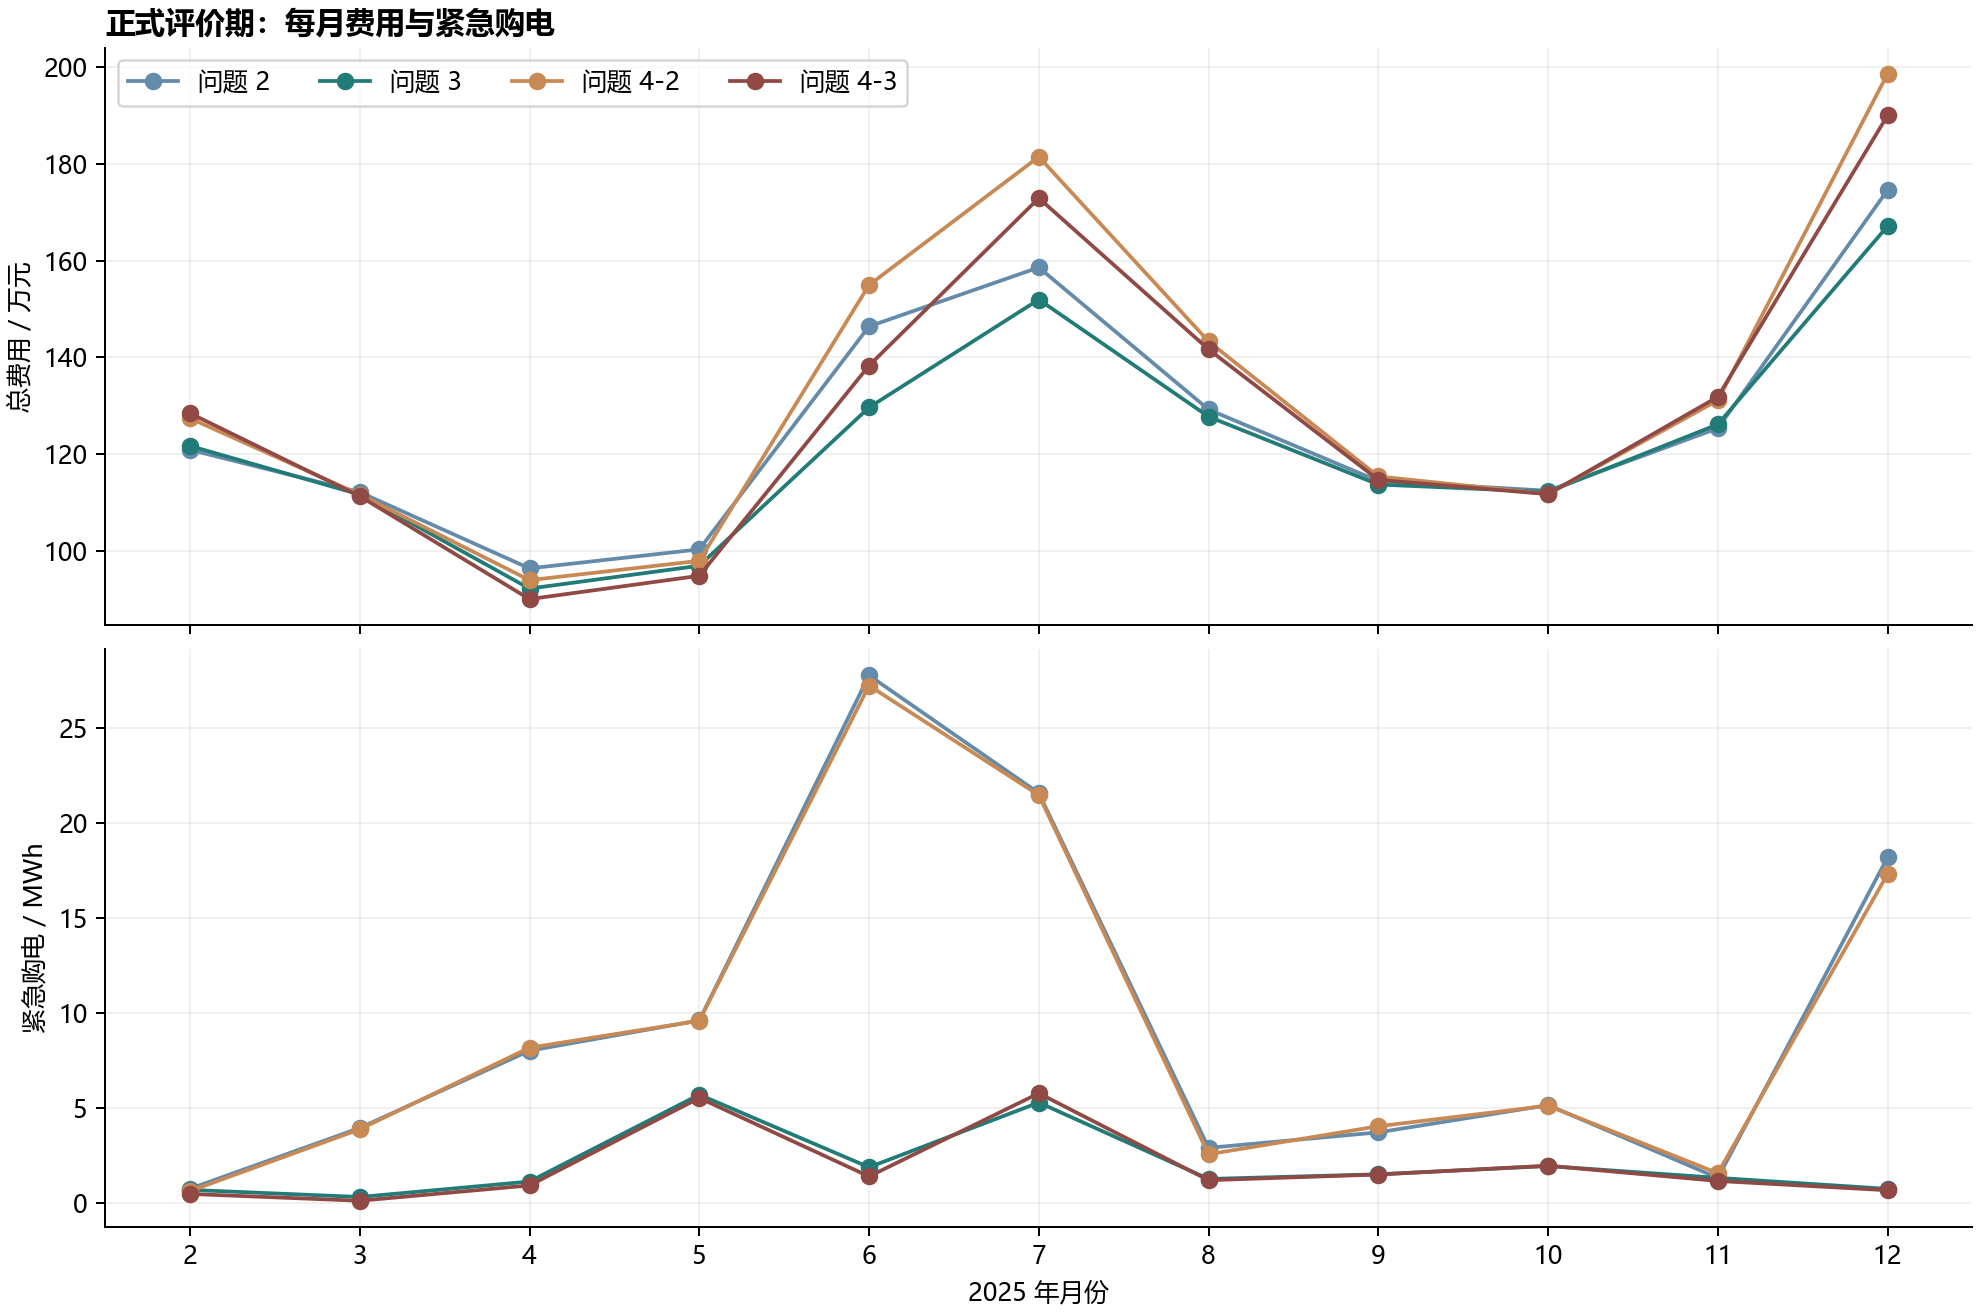
\includegraphics[width=\textwidth]{../outputs/figures/monthly-comparison.png}
 \caption{四种主方案在正式期各月的总购电费用与紧急购电量}\label{fig:monthly}
\end{figure}
3月20日、6月21日、9月23日、12月21日的指定购电时段、四小时充放电、全天费用与紧急事件完整列于附录\ref{app:days}。日内方案同时列原计划与最终常规购电；最终常规购电不含紧急电。不能将原计划费与“原计划费加调整费”再次相加。
\FloatBarrier

\subsection{历史光伏与纯附件三基准}
仅证明带日内调整的方案优于问题二不足以说明预测器有效。为此对纯历史光伏、纯附件三及两者融合均按相同1月评分区间选参，并用共同热启动比较正式期费用。
% Generated by scripts/build_paper_tables.py; do not edit by hand.
\par
\begin{table}[htbp]
\centering
\caption{共同热启动下的预测策略比较（2—12月）}\label{tab:forecast-baselines}
\small
\setlength{\tabcolsep}{4pt}
\renewcommand{\arraystretch}{1.15}
\begin{tabular}{lrrrrr}
\toprule
方案 & 光伏预测 & $\lambda$ & $\alpha$ & 费用（元） & 紧急电（kWh） \\
\midrule
问题3 & 纯附件3 & 1 & 0.65 & 13,511,208.12 & 21,565.68 \\
问题3 & 纯历史 & 0 & 0.65 & 13,428,215.91 & 38,224.16 \\
问题3 & 融合主方案 & 0.5 & 0.65 & 13,315,835.99 & 25,862.57 \\
问题4-3 & 纯附件3 & 1 & 0.65 & 14,258,363.92 & 20,483.78 \\
问题4-3 & 纯历史 & 0 & 0.65 & 14,166,961.16 & 38,253.28 \\
问题4-3 & 融合主方案 & 0.5 & 0.65 & 14,044,885.25 & 24,227.41 \\
\bottomrule
\end{tabular}
\par\smallskip
\begin{minipage}{0.97\linewidth}\footnotesize 各问题内的比较共用1月热启动及正式期初库存。各预测器依据同一1月准则选参，费用差是策略组合之差。\end{minipage}
\end{table}
\par

融合主方案相对共同热启动的历史基准，在问题三节省112379.91元，在问题4-3节省122075.92元；纯附件三在本数据上反而更贵。由此采用融合而非完全依赖附件三。但上述差值比较了经选参的预测与控制组合，仍包含风险残差和后续库存轨迹变化。

\subsection{新增小时光伏预报的严格子集对照}
为隔离新增小时预报，固定主预测器参数、规划器和反馈规则，保留06、12、18点三次重规划、当时真实库存、负荷修正及当前光伏观测锚点，仅改变允许读取的新小时预报集合。未读取时沿用最近可用发布行，并按相同绝对目标整点对齐。每种信息集合独立构造因果残差并连续运行。表中直接列出允许读取的新预报时刻，融合策略各子集共用1月热启动；纯附件三列用于展示原预测器下的同类对照。
% Generated by scripts/build_paper_tables.py; do not edit by hand.
\par
\begin{table}[htbp]
\centering
\caption{问题3新小时光伏预报的完整子集对照}\label{tab:hourly-subsets}
\small
\setlength{\tabcolsep}{4pt}
\renewcommand{\arraystretch}{1.15}
\begin{tabular}{lrrr}
\toprule
新增预报时刻 & 纯附件3费用（元） & 融合策略费用（元） & 融合紧急电（kWh） \\
\midrule
无 & 13,580,285.75 & 13,333,061.82 & 29,178.88 \\
18 & 13,580,285.30 & 13,333,062.82 & 29,178.86 \\
12 & 13,564,801.30 & 13,344,238.23 & 29,324.32 \\
12、18 & 13,564,801.43 & 13,344,238.54 & 29,324.42 \\
06 & 13,585,837.75 & 13,335,964.19 & 25,744.14 \\
06、18 & 13,585,837.09 & 13,335,963.52 & 25,744.09 \\
06、12 & 13,511,207.99 & 13,315,835.68 & 25,862.47 \\
06、12、18 & 13,511,208.12 & 13,315,835.99 & 25,862.57 \\
\bottomrule
\end{tabular}
\par\smallskip
\begin{minipage}{0.97\linewidth}\footnotesize 各行均保留06、12、18点重规划、实际SOC、负载修正及当前光伏观测锚点；仅开关新小时预报。融合子集共用1月热启动。\end{minipage}
\end{table}
\par

全部允许相对全部不读取，正式费用减少17225.82元。分别从完整集合去掉06点、12点或18点新小时预报，费用变化为$+28402.55$元、$+20127.52$元与$-0.31$元。这些边际量有交互作用，不能直接求和；18点的量级不能支持可辨认的经济增益。

若连重规划机会一并取消，会同时失去调整库存、修正负荷和提前增购的能力。允许全部重规划相对仅零时规划的费用差为745563.95元，属于整体策略效果。故“18点新光伏预报没有可辨认的改善”不等于“18点调整购电没有价值”。
\FloatBarrier
